
\chapter{Momentum
}
\begin{frame}
  La segunda ley de Newton en su forma más general puede escribirse, para una partícula de moméntum $\mathbf{p}$, como (ver ec.~(\ref{eq:28})
\begin{align}
  \mathbf{F}=\frac{d\mathbf{p}}{dt}\,.
\end{align}
Demostraremos que en la ecuación anterior cuando es aplicada a un sistéma de partículas, sólo contribuyen las fuerzas externas. 
\end{frame}

\section{Dinámica de un sistema de partículas}
Considere un sistema de $N$ partículas interactuantes con masas $m_1$, $m_2$, $m_3$, $\ldots$, $m_N$. La posición de la $i$-sima partícula es $\mathbf{r}_i$, y la fuerza sobre esta es $\mathbf{F}_i$. La ecuación de movimiento de la $i$-sima partícula es
\begin{align}
  \mathbf{F}_i=\frac{d\mathbf{p}_i}{dt}
\end{align}
Las fuerza sobre la partícula $i$ puede desdoblarse en dos términos
\begin{align}
  \mathbf{F}_i=\mathbf{F}_i^{\text{int}}+\mathbf{F}_i^{\text{ext}}\,.
\end{align}
Aquí $\mathbf{F}_i^{\text{int}}$, la fuerza \emph{interna} sobre la partícula $i$, es la fuerza debida a todas las partículas dentro del sistema, y $\mathbf{F}_i^{\text{ext}}$, la fuerza externa sobre la partícula $i$, es decir la fuerza debida a fuentes externas al sistema. La ecuación de movimiento es entonces
\begin{align}
  \mathbf{F}_i^{\text{int}}+\mathbf{F}_i^{\text{ext}}=\frac{d\mathbf{p}_i}{dt}\,.
\end{align}

El resultado de sumar todas las ecuaciones de movimiento para cada una de las partículas es entonces
\begin{align}
  \label{eq:msumfi}
  \sum_{i=1}^N  \mathbf{F}_i^{\text{int}}+\sum_{i=1}^N\mathbf{F}_i^{\text{ext}}=\sum_{i=1}^N \frac{d\mathbf{p}_i}{dt}\,.
\end{align}
El segundo término corresponde a todas las fuerzas externas actuando sobre todas las partículas. Ésta es la fuerza externa total, $\mathbf{F}_{\text{ext}}$, actuando sobre el sistema
\begin{align}
 \mathbf{F}_{\text{ext}}=& \sum_{i=1}^N\mathbf{F}_i^{\text{ext}}\,.
\end{align}
El primer término en la ec.~(\ref{eq:msumfi}), es la suma de todas las fuerzas internas actuando sobre todas las partículas. De acuerdo a la tercera ley de Newton, las fuerzas entre cualquier  par de partículas son iguales y opuestas de modo que su suma es cero. Se sigue que la suma de las fuerzas entre todas las partículas también es cero, de modo que las fuerzas internas se cancelan a pares. De aquí
\begin{align}
\sum_{i=1}^N  \mathbf{F}_i^{\text{int}}=&0\,.  
\end{align}

La ec.~(\ref{eq:msumfi}) se simplifica a
\begin{align}
  \label{eq:mfext}
  \mathbf{F}_{\text{ext}}=&\sum_{i=1}^N \frac{d\mathbf{p}_i}{dt}\nonumber\\
  =& \frac{d}{dt}\sum_{i=1}^N\mathbf{p}_i\nonumber\\
 \mathbf{F}_{\text{ext}} =& \frac{d}{dt}\mathbf{P}\,,
\end{align}
donde
\begin{align}
  \mathbf{P}=\sum_{i=1}^N\mathbf{p}_i\,,
\end{align}
es el moméntum total del sistema. De modo que la fuerza externa
aplicada a un sistema es igual a la tasa de cambio del momentum total del sistema. Esto es cierto independiente de los detalles de la interacción. $\mathbf{F}_{\text{ext}}$ podría ser una sola fuerza actuando en una sola partícula, o podría ser la resultante de muchas interacciones involucrando cada una de las partículas del sistema.

En adelante omitiremos el subíndice ext de la ec.~(\ref{eq:mfext}), de modo que
\begin{align}
  \label{eq:mfdpdt}
  \mathbf{F}=&\frac{d\mathbf{P}}{dt}\,.
\end{align}
El resultado es idéntico a la ecuación de movimiento para una sola partícula, aunque de hecho se refiere a un sistema de partículas. 


\section{Centro de masa}


Sea un conjunto de partículas con cantidades de movimientos diferentes formando un sistema que ocupa una región del espacio. En un instante en particular el sistema se vería como el que se ilustra en la figura~\ref{fig:centrodemasa}
\begin{frame}
  \begin{figure}
  \centering
%\only<1>{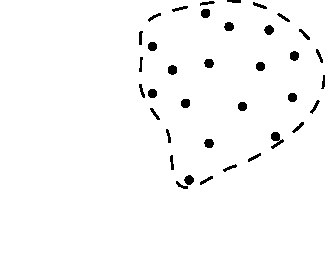
\includegraphics[scale=1.3]{centrodemasa0}}%
%\only<2>{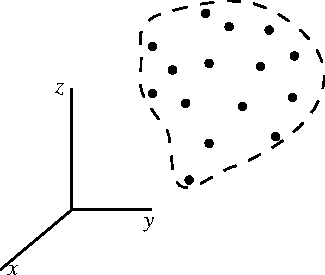
\includegraphics[scale=1.3]{centrodemasa1}}%
%\only<3>{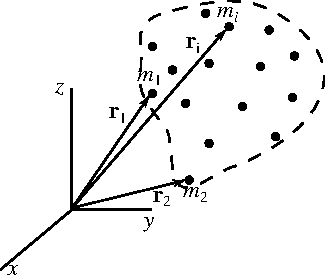
\includegraphics[scale=1.3]{centrodemasa2}}%
%\only<4>%
{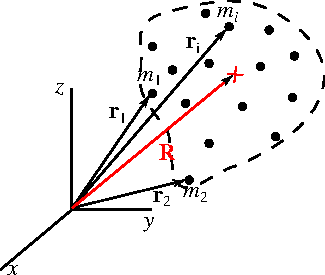
\includegraphics[scale=1.3]{centrodemasa3}}
  \caption{Centro de masa}
  \label{fig:centrodemasa}
\end{figure}
\end{frame}

Si consideremos el sistema en su totalidad con una masa
\begin{align}
  M=\sum_{i=1}^N m_i\,,
\end{align}
podemos intentar escribir la ecuación de movimiento en la forma especial de masa constante
\begin{align}
    \mathbf{F}=&\frac{d\mathbf{P}}{dt}\nonumber\\
    \mathbf{F}=&\sum_{i=1}^N\frac{d\mathbf{p}_i}{dt}\nonumber\\
    \mathbf{F}=&\sum_{i=1}^N\frac{d(m_i\mathbf{v}_i)}{dt}\nonumber\\
    \mathbf{F}=&\sum_{i=1}^Nm_i\frac{d\mathbf{v}_i}{dt}\nonumber\\
    \mathbf{F}=&\sum_{i=1}^Nm_i\frac{d\dot{\mathbf{r}}_i}{dt}\,,
\end{align}
que podemos escribir en la forma
\begin{align}
  \label{eq:mcm}
  \mathbf{F}=M\ddot{\mathbf{R}}\,,
\end{align}
si
\begin{align}
  M\ddot{\mathbf{R}}=\frac{d\mathbf{P}}{dt}=&\frac{d}{dt}\sum_{i=1}^N m_i\dot{\mathbf{r}}_i\nonumber\\
=&\sum_{i=1}^N m_i\ddot{\mathbf{r}}_i\,,
\end{align}
con $\mathbf{r}_i$ el vector de posición de cada una de las partículas con respecto a un sistema de coordenadas. Entonces
\begin{align}
\label{eq:mveccm}
  \ddot{\mathbf{R}}=\frac{1}{M}\sum_{i=1}^Nm_i\ddot{\mathbf{r}}_i\,.
\end{align}
Integrando formalmente dos veces
\begin{align}
  \int_0^{\dot{\mathbf{R}}}d(\dot{\mathbf{R}})=&\frac{1}{M}
  \sum_{i=1}^N m_i\int_0^{\dot{\mathbf{r}}_i}d(\dot{\mathbf{r}}_i)\nonumber\\
  \dot{\mathbf{R}}=&\frac{1}{M}
  \sum_{i=1}^N m_i\dot{\mathbf{r}}_i\,,\nonumber\\
  \int_0^{{\mathbf{R}}}d({\mathbf{R}})=&\frac{1}{M}
  \sum_{i=1}^N m_i\int_0^{{\mathbf{r}}_i}d({\mathbf{r}}_i)\nonumber\\
  {\mathbf{R}}=&\frac{1}{M}
  \sum_{i=1}^N m_i{\mathbf{r}}_i\,.
\end{align}

Definido de esta forma $\mathbf{R}$ es un vector desde el origen de coordenadas a un punto llamado el \emph{centro de masa} del sistema, como se ilustra en la figura~\ref{fig:centrodemasa}. El sistema se comporta como si toda la masa está concentrada en el centro de masa y todas las fuerzas externas actuaran sobre ese punto.

Muchas veces estamos interesados en el movimiento de cuerpos relativamente rígidos como pelotas o automóviles. Cuerpos de esta índole, corresponden a sistemas de partículas que están fijas entre sí por fuertes fuerzas internas. La ec.~(\ref{eq:mveccm}) muestra que con respecto a fuerzas externas, el cuerpo se comporta como si fuera una partícula virtual. En el capítulo~\ref{cha:dinamica}, casualmente tratamos cada cuerpo como si fuesen partículas; vemos ahora que esto esta justificado con tal que centremos nuestra atención en el movimiento del centro de masa. 

La ecuación~(\ref{eq:mcm}) es solo válida para estudiar la traslación del centro de masa. En ausencia de fuerzas externas, la aceleración del centro de masa es cero, de modo que $\ddot{\mathbf{R}}=0$, es decir, el centro de masa se mueve a velocidad constante. Esta ley de conservación proviene de la invarianza de los sistemas bajo transformaciones de Galileo

Ilustración del movimiento de centro de masa: \url{http://www.wired.com/wiredscience/2011/09/modeling-a-falling-slinky/}. Simulación y código  \href{http://www.wired.com/wiredscience/2011/10/more-slinky-physics/}{con una pelota de tenis en el extermo}

\begin{itemize}
\item[\textbf{Ejemplo:}] Calcule el centro de masa de masa de un par de esferas de masa $m_1$ y $m_2$ unidas por una varilla de masa despreciable como se muestra en la figura~\ref{fig:varilla}. Ver
  \begin{align}
    \label{eq:mbaton}
    \mathbf{R}=\frac{m_1\mathbf{r}_1+m_2\mathbf{r}_2}{m_1+m_2}
  \end{align}
Note que la línea que une los extremos de los vectores de posición $\mathbf{r}_1$ y $\mathbf{r}_2$ corresponde a la diferencia $\mathbf{r}_1-\mathbf{r}_2$. Para comprobar que $\mathbf{R}$ se encuentra sobre esa línea,
sea el desplazamiento desde la punta de $\mathbf{R}$ hasta la punta $\mathbf{r}_1$ el vector $\mathbf{r}_1'$ como se muestra en la figura~\ref{fig:varilla}. De la misma forma, sea $\mathbf{r}_2'$ el vector de desplazamiento entre los extremos de $\mathbf{R}$ y $\mathbf{r}_2$. Entonces
\begin{align}
  \mathbf{r}_1'=&\mathbf{r}_1-\mathbf{R}\nonumber\\
  \mathbf{r}_2'=&\mathbf{r}_2-\mathbf{R}\,.
\end{align}
De la ec.~\eqref{eq:mbaton}
\begin{align}
  \mathbf{r}_1'=&\mathbf{r}_1-\mathbf{R}\nonumber\\
  =&\mathbf{r}_1-\frac{m_1\mathbf{r}_1+m_2\mathbf{r}_2}{m_1+m_2}\nonumber\\
    =&\frac{\mathbf{r}_1(m_1+m_2)-m_1\mathbf{r}_1-m_2\mathbf{r}_2}{m_1+m_2}\nonumber\\
    =&\frac{m_2}{m_1+m_2}(\mathbf{r}_1-\mathbf{r}_2)\,,
\end{align}
de modo que el vector $\mathbf{r}_1$ es paralelo a la varilla que une las dos esferas determinada por $\mathbf{r}_1-\mathbf{r}_2$. Similarmente
\begin{align}
  %faltan detalles
 \mathbf{r}_2'=-\left(\frac{m_1}{m_1+m_2} \right)\left(\mathbf{r}_1-\mathbf{r}_2 \right)\,.
\end{align}
De modo que tanto $\mathbf{r}_1'$ como $\mathrm{r}_2'$ yacen sobre la línea que une $m_1$ y $m_2$. Además, si la longitud de dicha línea es $l$
\begin{align}
  r_1'=&\frac{m_2}{m_1+m_2}l\nonumber\\
  r_2'=&\frac{m_1}{m_1+m_2}l\,.
\end{align}

Asumiendo que la fricción es despreciable, la fuerza externa sobre el cuerpo cuando es lanzado al aire es
\begin{align}
  \mathbf{F}=m_1\mathbf{g}+m_2\mathbf{g},
\end{align}
donde
\begin{align}
  \mathbf{g}=-g\hat{\mathbf{j}}\,.
\end{align}
La ecuación de movimiento para el centro de masa es:
\begin{align*}
  \mathbf{F}=&m_1\frac{d\dot{\mathbf{r}}_1}{dt}+m_2\frac{d\dot{\mathbf{r}_2}}{dt}\nonumber\\
=&m_1(\ddot{\mathbf{r}}_1'+\ddot{\mathbf{R}})+m_2(\ddot{\mathbf{r}}_2'+\ddot{\mathbf{R}})\nonumber\\
=&(m_1+m_2)\ddot{\mathbf{R}})+\frac{m_1m_2}{m_1+m_2}(\mathbf{r}_1-\mathbf{r}_2)
                            -\frac{m_1m_2}{m_1+m_2}(\mathbf{r}_1-\mathbf{r}_2)\nonumber\\
=&(m_1+m_2)\ddot{\mathbf{R}}
\end{align*}
de modo que
\begin{align}
  \left(m_1+m_2 \right)\ddot{\mathbf{R}}=\left(m_1+m_2 \right)\mathbf{g}\,,
\end{align}
o
\begin{align}
  \ddot{\mathbf{R}}=\mathbf{g}\,.
\end{align}
El centro de masa sigue la trayectoria parabólica de una sola masa.
\end{itemize}

\begin{frame}
  \begin{figure}
    \centering
%\only<1>%
{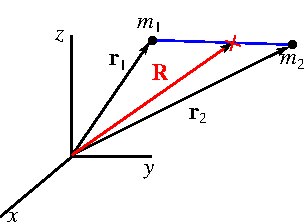
\includegraphics[scale=1.3]{varilla0}}
%\only<2>%
{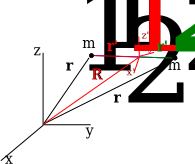
\includegraphics[scale=1.3]{varilla1}}
    \caption{Barra}
    \label{fig:varilla}
  \end{figure}
\end{frame}
Para cuerpos continuos es más conveniente hacer una integral:
%faltan detalles
\begin{align}
  \mathbf{R}=\frac{1}{M}\int \mathbf{r} dm\,.
\end{align}

Para visualizar esta integral, piense en $dm$ como la masa de un elemento de volumen $dV$ localizada en la posición $\mathbf{r}$, como se muestra en la figura~\ref{fig:centrodemasacontinuo}. Si la densidad de masa del elemento es $\rho$, entonces $dm=\rho\,dV$, y
\begin{align}
\label{eq:mintvol}
  \mathbf{R}=\frac{1}{M}\int_V \mathbf{r}\,\rho\,dV\,, 
\end{align}
donde
\begin{align}
  \mathbf{r}=x\hat{\mathbf{i}}+y\hat{\mathbf{j}}+z\hat{\mathbf{k}}\,.
\end{align}
La integral en (\ref{eq:mintvol}), es llamada una integral de volumen.

\begin{frame}
  \begin{figure}
  \centering
  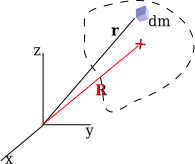
\includegraphics[scale=1.3]{centrodemasacontinuo}
  \caption{Centro de masa continuo}
  \label{fig:centrodemasacontinuo}
\end{figure}
\end{frame}

\begin{itemize}
\item[\textbf{Ejemplo}] \textbf{Centro de masa de una varilla no uniforme}: Calcular el centro de masa de una varilla de densidad lineal $\lambda=\lambda_0(x/L)$, donde $L$ es la longitud de la varilla
  \begin{align}
    \mathbf{R}=&\frac{1}{M}\int \mathbf{r}\lambda\,dx\,.
  \end{align}
Teniendo en cuenta que
\begin{align}
  \mathbf{r}=&(x,0,0)\nonumber\\
  \mathbf{R}=&(R_x,0,0)\,,
\end{align}
tenemos que
\begin{align}
  \label{eq:m38}
  R_x=&\frac{1}{M}\int_0^L x\lambda(x)dx\nonumber\\
  =&\frac{1}{M}\frac{\lambda_0}{L}\int_0^L x^2\,dx\,.
\end{align}
Debemos calcular $M$:
\begin{align}
  M=\int dm=\frac{\lambda_0}{L}\int_0^L x\,dx=\frac{\lambda_0}{L}
  \left.\frac{x^2}{2}  \right|_0^L=\frac{\lambda_0}{2}L\,.
\end{align}
Reemplazando en \eqref{eq:m38}
\begin{align}
  R_x=&\frac{2}{\lambda_0L}\frac{\lambda_0}{L}\int_0^L x^2\,dx\nonumber\\
  =&\frac{2}{L^2}\left.\frac{x^3}{3}  \right|_0^L\nonumber\\
  =&\frac{2}{L^2}\frac{L^3}{3}\nonumber\\
  =&\frac{2}{3}L\,.
\end{align}

\item[\textbf{Ejemplo}] \textbf{Centro de masa de una hoja triangular} 
\end{itemize}

\section{Conservación del momentum}
Para un sistema aislado, es decir, un sistema que no interactúa con sus alrededores se tiene que $\mathbf{F}=0$, y por lo tanto
\begin{align}
  \frac{d\mathbf{P}}{dt}=0\,.
\end{align}
De modo que el momentum total es constante, sin importar que tan fuerte son las interacciones internas, y sin importar lo complicado del movimiento. Esta es la ley de conservación del momentum.

\begin{itemize}
\item[\textbf{Ejemplo}] \textbf{Retroceso de un cañón de resorte}\\
Un cañón de resorte cargado, inicialmente en reposo en una superficie horizontal sin fricción, dispara una canica con un ángulo de elevación $\theta$. La masa del cañón es $M$, la masa de la canica es $m$, y la velocidad de salida de la canica es $v_0$ relativa al cañón. ¿Cual es la velocidad final del cañon?

Considere el sistema como compuesto por el cañón más la canica. Como la gravedad y la fuerza son verticales no existen fuerzas horizontales en la dirección $x$, de modo que
\begin{align}
  \frac{d P_x}{dt}=0,.
\end{align}
Como $P_x$ se conserva:
\begin{align}
  P_{x,\text{inicial}}=P_{x,\text{final}}
\end{align}
Sea el tiempo inicial anterior a disparar el cañón. Entonces $P_{x,\text{inicial}}=0$, ya que el sistema está inicialmente en reposo. Después de que la canica ha abandonado la boca del cañón, el cañón retrocede con alguna rapidez $V_f$, y su momentum final es $M V_f$ hacia la izquierda. La velocidad de la canica relativa a la  mesa es $v_0\cos\theta-V_f$. Por conservación del momentum horizontal, tenemos por consiguiente que
\begin{align}
  0=m(v_0\cos\theta-V_f)-M V_f\,,
\end{align}
o
\begin{align}
  V_f=\frac{m v_0\cos\theta}{M+m}\,.
\end{align}

\end{itemize}

\begin{frame}
  \begin{figure}
    \centering
%\only<1>%
{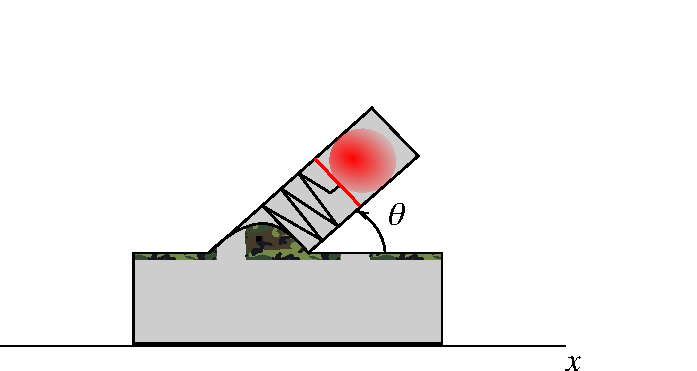
\includegraphics[scale=0.7]{canon0}}
%\only<2>%
{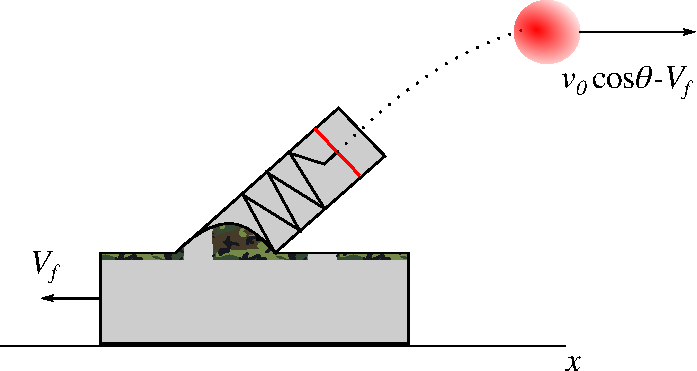
\includegraphics[scale=0.7]{canon1}}
    \caption{Cañón}
    \label{fig:canon}
  \end{figure}
\end{frame}

% \begin{itemize}
% \item[\textbf{Ejemplo}] \textbf{Rebote de pelota de goma}
% \end{itemize}

\section{Sistemas de masa variable}
Para este tipo de sistemas se debe usar
\begin{align}
  \mathbf{F}=\frac{d\mathbf{P}}{dt}\,.
\end{align}

Para analizar este tipo de sistemas es esencial tratar con el mismo conjunto de partículas a través de todo el intervalo temporal desde el tiempo inicial al tiempo final; debemos rastrear todas las partículas que estaban originalmente en el sistema. Consecuentemente, la masa del sistema no puede cambiar durante el intervalo de interés. En el caso de un cohete, el sistema está compuesto por el cohete en sí, y el combustible que tenga al momento inicial. 



Considere un cohete a un tiempo $t$ que se mueve a velocidad $\mathbf{v}$. Entre un tiempo $t$ y $t+\Delta t$, una masa de combustible $\Delta m$ es quemada y expulsada como gas a una velocidad $\mathbf{u}$ relativa al cohete.

El sistema consiste de $\Delta m$ más la masa remanente del cohete $M$. De aquí que la masa total es $M+\Delta m$.

La velocidad del cohete al tiempo $t$ es $\mathbf{v}(t)$, y en $t+\Delta t$, es $\mathbf{v}+\Delta\mathbf{v}$. Similarmente, la velocidad de la masa de combustible al tiempo $t$ es $\mathbf{v}(t)$, y al tiempo $t+\Delta t$, es la velocidad del cohete a ese tiempo, más la suma vectorial de su propia velocidad: $\mathbf{v}+\Delta\mathbf{v}+\mathbf{u}$. 

El momentum inicial es:
\begin{align}
  \mathbf{P}(t)=(M+\Delta m)\mathbf{v}\,,
\end{align}
y el momentum final es
\begin{align}
  \mathbf{P}(t+\Delta t)=M(\mathbf{v}+\Delta\mathbf{v})+\Delta m(\mathbf{v}+\Delta\mathbf{v}+\mathbf{u})\,.
\end{align}
El cambio en el momentum es
\begin{align}
  \Delta\mathbf{P}=&\mathbf{P}(t+\Delta t)-\mathbf{P}(t)\nonumber\\
=&M\Delta\mathbf{v}+(\Delta m)(\Delta\mathbf{v})+(\Delta m)\mathbf{u}\nonumber\\
\approx &M\Delta\mathbf{v}+(\Delta m)\mathbf{u}\,,
\end{align}
donde hemos despreciado el producto de términos pequeños. Por consiguiente
\begin{align}
  \frac{d\mathbf{P}}{dt}=&\lim_{\Delta t\to 0}\frac{\Delta\mathbf{p}}{\Delta t}\nonumber\\
=&M\frac{d\mathbf{v}}{dt}+\mathbf{u}\frac{dm}{dt}\,.
\end{align}
$dm/dt$ es la tasa de cambio de la masa expulsada. Ya que esta masa proviene del cohete
\begin{align}
  \frac{dm}{dt}=-\frac{dM}{dt}\,,
\end{align}
y
\begin{align}
  \frac{d\mathbf{P}}{dt}=M\frac{d\mathbf{v}}{dt}-\mathbf{u}\frac{dM}{dt}\,.
\end{align}
como
\begin{align}
  \mathbf{F}_{\text{ext}}=\frac{d\mathbf{P}}{dt},,
\end{align}
entonces
\begin{align}
  \label{eq:mrocket}
   \mathbf{F}_{\text{ext}}=M\frac{d\mathbf{v}}{dt}-\mathbf{u}\frac{dM}{dt}\,.
\end{align}
Esta es la ecuación de movimiento para un cohete en presencia de
fuerzas externas

\subsection{Cohete en el espacio libre}

En el espacio exterior en ausencia de gravedad no hay fuerzas externas actuando sobre el cohete, de modo que $\mathbf{F}=0$ y la ecuación de movimiento~(\ref{eq:mrocket}) esta dada por
\begin{align}
\label{eq:m40}
  \mathbf{F}_{\text{ext}}=0\Longrightarrow M\frac{d\mathbf{v}}{dt}=\mathbf{u}\frac{dM}{dt}\,,
\end{align}
Definimos la fuerza de empuje del cohete como
\begin{align}
  \label{eq:m39}
  \mathbf{F}_E=M\frac{d\mathbf{v}}{dt}=\mathbf{u}\frac{dM}{dt}\,.
\end{align}

La ec.~\eqref{eq:40} puede reescribirse como
\begin{align}
  \label{eq:m41}
  \frac{d\mathbf{v}}{dt}=\mathbf{u}\frac{1}{M}\frac{dM}{dt}\,.
\end{align}


Generalmente la velocidad de expulsión $\mathbf{u}$ es constante, en tal caso es fácil integrar la ecuación de movimiento:
\begin{align}
{d\mathbf{v}}=\mathbf{u}\frac{dM}{M}\,.
\end{align}
La antiderivada de $1/x$ es $\ln x$, ya que
\begin{align}
  \frac{d}{dx}\ln x=\frac{1}{x},.
\end{align}
Asumiendo que $\mathbf{u}$ es constante en magnitud y dirección,
entonces
\begin{align}
  \int_{\mathbf{v}_0}^{\mathbf{v}_f}{d\mathbf{v}}=&\mathbf{u}\int_{M_0}^{M_f}\frac{dM}{M}\nonumber\\
\mathbf{v}_f-\mathbf{v}_0=&\mathbf{u}\ln M\left|_{{}_{M_0}}^{{}^{M_f}}\right.\nonumber\\
=&\mathbf{u}\left(\ln M_f-\ln M_0\right)\nonumber\\
=&\mathbf{u}\ln\frac{M_f}{M_0}\nonumber\\
=&-\mathbf{u}\ln\frac{M_0}{M_f}\,.
\end{align}

Si $\mathbf{v}_0=0$, entonces
\begin{align}
  \mathbf{v}_f=&-\mathbf{u}\ln\frac{M_0}{M_f}\,.
\end{align}
La velocidad final es independiente de como la masa es liberada. Las únicas cantidades importante son las velocidades de expulsión y el cociente entre las masas finales e iniciales.

\begin{itemize}
\item[\textbf{Ejemplo}]Si un cohete de masa $M=\unit{1000}{\kilo\gram}$ está expulsando gas a una tasa de $\unit{10}{\kilo\gram\per\second}$, y a una velocidad de expulsión de $\unit{500}{\meter\per\second}$. Calcule la velocidad después de $\unit{20}{\second}$.\\
Después de $\unit{20}{\second}$ el cohete a expulsado una masa de $\unit{10}{\kilo\gram\per\second}\timesm\unit{20}{\second}=\unit{200}{\kilo\gram}$, de modo que $M_f=\unit{1000}{\kilo\gram}-\unit{200}{\kilo\gram}=\unit{800}{\kilo\gram}$, entonces
\begin{align}
  v_f=(-\unit{500}{\meter\per\second})\ln\frac{800}{1000}=\unit{112}{\meter\per\second}\,.
\end{align}
Del enunciado del problema se puede 
\begin{align}
  \frac{dM}{dt}=-10\ \frac{\text{Kg}}{\text{s}}\,,
\end{align}
donde el signo menos indica que la masa total del sistema cohete--combustible esta disminuyendo con el tiempo. Integrando entre un tiempo $t_i=0$ y un tiempo final $t$, tenemos
\begin{align}
  \int_0^t dM&=-10\int_0^t\nonumber\\
  M(t)&=-M(0)-10 t
\end{align}
Usando el valor para la masa inicial $M(0)=\unit{1000}{\kilo\gram}$, tenemos
\begin{align*}
  M(t)=&\unit{(1000-10t)}{\kilo\gram}\nonumber\\
  \frac{dM(t)}{dt}=&-10\kilo\gram\per\second
\end{align*}
Usando la ec.~\eqref{eq:m39} podemos calcular el empuje del cohete:
\begin{align}
  \mathbf{F}_E=\mathbf{u}\frac{dM}{dt}=&\mathbf{u}(-10)\nonumber\\
  =&(-500)\timesm(-10)\hat{\mathbf{i}}\nonumber\\
  =&{5000}{\newton}\,\hat{\mathbf{i}}\,,
\end{align}
y  el empuje producido por el cohete es de ${5000}{\newton}$,  
\end{itemize}

%\begin{inprogress}
%http://mypages.iit.edu/~smart/acadyear/rockets.htm
y la aceleración
\begin{align}
  \mathbf{a}=&\frac{\mathbf{F}_E}{M(t)}\nonumber\\
  =&\unit{\frac{5000}{1000-10t}}{\meter\per\second\squared}\,\hat{\mathbf{i}}\nonumber\\
  =&\unit{\frac{500}{100-t}}{\meter\per\second\squared}\,\hat{\mathbf{i}}
\end{align}
de modo que
\begin{align}
  \textbf{v}=\unit{[-500\ln(-100+t)]}{\meter\per\second}\,\hat{\mathbf{i}}
\end{align}
\begin{align}
 \mathbf{x}=\unit{\{-500 [-t+t \ln (t-100)-100 \ln (100-t)]\}}{\meter}\,\hat{\mathbf{i}}
\end{align}
%\end{inprogress}


Si el cohete está en presencia de un campo gravitacional constante (cerca a la superficie de la tierra), la fuerza externa es
\begin{align}
  \mathbf{F}=M\mathbf{g}
\end{align}
y de \eqref{eq:mrocket}
\begin{align}
     M\mathbf{g}=M\frac{d\mathbf{v}}{dt}-\mathbf{u}\frac{dM}{dt}\,,
\end{align}
de donde
\begin{align}
  \frac{d\mathbf{v}}{dt}=\frac{\mathbf{u}}{M}\frac{dM}{dt}+\mathbf{g}\,.
\end{align}
Integrando como en la ec.~\eqref{eq:m41}
\begin{align}
   \int_{\mathbf{v}_0}^{\mathbf{v}_f}{d\mathbf{v}}=&
   -\mathbf{u}\ln\frac{M_0}{M_f}+\mathbf{g}(t_f-t_0)
\end{align}






\section{Impulso}
\begin{frame}
  %\begin{block}%
{Definición de impulso:}
\begin{align}
  \text{Impulso}=\mathbf{F}_{\text{neta}}\Delta t
\end{align}
en unidades SI de $\text{N}\cdot\text{s}$ (newton-segundo)
  %\end{block}
\end{frame}

Con esta definición del impulso podemos establecer el Principio de Moméntum en las siguientes palabras:
\begin{frame}
  \begin{center}
    \textbf{El cambio de moméntum de un sistema es igual al impulso aplicado a éste.}
  \end{center}
\end{frame}

Ejemplo: Una fuerza constante de $(3,-5,4)\ $N actúa en un objeto durante $10\ $s. ¿Cuál es el impulso neto aplicado al objeto? ¿Cual fue el cambio en el momentum del objeto?
\begin{align}
\text{Impulso}=\mathbf{F}_{\text{neta}}\Delta t=(3,-5,4)\ \text{N}\cdot (10\ \text{s})=
(30,-50,40)\ \text{N}\cdot\text{s}\,.
\end{align}
El cambio en el moméntum del objeto es igual al impulso neto, de modo que
\begin{align}
  \Delta \mathbf{p}=(30,-50,40)\ \text{Kg\,m/s}
\end{align}

durante un intervalo suficientemente pequeño $\Delta t=t_b-t_a$, tenemos
\begin{align}
   \mathbf{I}=\mathbf{F}\Delta t=&\mathbf{P}(t_b)-\mathbf{P}(t_a)\,.
\end{align}

\subsection{Transporte de momomentum}

El empuje de un chorro de agua proviene del moméntum que transfiere, por ejemplo sobre una pared. ¿Cómo puede una columna de agua transmitir una fuerza tan real como la de una varilla de hierro?. La razón es fácil de ver si nos imaginamos el chorro de agua como una serie de pequeñas gotas de masa uniforme $m$, viajando a una velocidad $v$.  

Considere entonces, un chorro de partículas de masa $m$ y separación
$l$ que golpean perpendicularmente una superficie con rapidez $v$,
como se ilustra en la figura~\ref{fig:gotas}. El chorro rebota sobre
la misma línea original de movimiento con rapidez $v'$. La masa por
unidad de longitud del chorro incidente es $\lambda=m/l$.

\begin{frame}
 \begin{figure}
  \centering
%\only<1>%
{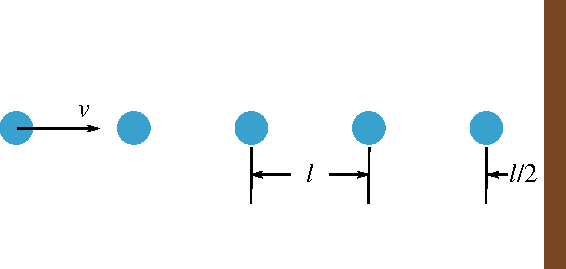
\includegraphics{gotas0}}
%\only<2>%
{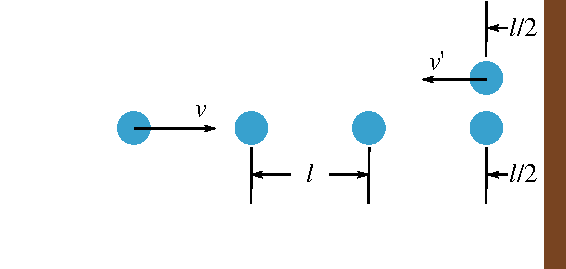
\includegraphics{gotas1}}
  \caption{Gotas golpeando un pared}
  \label{fig:gotas}
\end{figure}
\end{frame}
Para encontrar el impulso de una gota rebotando con rapides $v'$ sobre la pared, tenemos
%hacer grafico
\begin{align*}
  \int_{t_a}^{t_b} \mathbf{F} dt\approx \mathbf{F}_{\text{prom}}\Delta t=&\Delta \mathbf{p}\nonumber\\
=&m (\mathbf{v}'-\mathbf{v})\nonumber\\
=&m[v'\,\hat{\mathbf{i}}-v(-\hat{\mathbf{i}})]\nonumber\\
=&m(v'+v)\hat{\mathbf{i}}\,.
\end{align*}
es el impulso sobre la pared durante el intervalo $\Delta t$. Si escogemos el intervalo $\Delta t$, tal que la gota recorra una distancia $l$, entonces
\begin{align*}
  \Delta t=\frac{l}{v}
\end{align*}
y
\begin{align*}
  F_{\text{prom}}\frac{l}{v}=&m(v+v')\,,
\end{align*}
y despejando la fuerza promedio de las gotas sobre la pared, tenemos
\begin{align*}
    F_{\text{prom}}=&\frac{m}{l}v(v+v')\nonumber\\
  =&\frac{m}{l}v(v+v')\nonumber\\
  =&\lambda(v+v')\nonumber\\
\end{align*}
Si el chorro colisiona sin rebotar, entonces $v'=0$, y
\begin{align*}
F=\lambda v^2\,.  
\end{align*}
mientras que si rebotan $v'=v$
\begin{align*}
  F=2\lambda v^2\,,
\end{align*}
de nuevo el efecto karate.

\begin{borrar}
la fuerza promedio sobre la superficie de una gota, considere la longitud $L$ del chorro justo antes de comenzar a golpear la superficie. El número de gotas en $L$ es $L/l$, y ya que cada gota tiene moméntum $m v$, el momentum total es
\begin{align*}
  \Delta p=\frac{L}{l}m v\,.
\end{align*}
Todas estas gotas golpearán la pared en el tiempo
\begin{align*}
  \Delta t=\frac{L}{v}\,.
\end{align*}
%poner gradico de la fuerza promedio
La tasa a la cual las gotas transportan moméntum a la superficie es
\begin{align*}
  \frac{\Delta p}{\Delta t}
  =&\frac{\displaystyle\frac{L}{l}m v_0}{\displaystyle\frac{L}{v}}\nonumber\\
  =&\frac{m}{l}v^2\,.
\end{align*}


Para aplicar este modelo a un fluido, considere un chorro moviendo con velocidad $v$. Si la masa por unidad de longitud es $m/l\equiv \lambda$, el moméntum por unidad de longitud es $\lambda v$, y la tasa a la cual el chorro transporta moméntum a la superficie es
\begin{align*}
  \frac{dp}{dt}=\lambda v^2\,.
\end{align*}

Si el chorro rebota con velocidad $v'$ en la superficie, la fuerza sobre la superficie es
\begin{align*}
  F=\frac{dp'}{dt}+\frac{dp}{dt}=&\lambda {v'}^2+\lambda v^2\nonumber\\
  =&\lambda v'v'+\lambda v^2\nonumber\\
  =&\lambda v'v'+\lambda v^2\nonumber\\
  =&\lambda v (v'+v)\,.
\end{align*}

Si el chorro colisiona sin rebotar, entonces $v'=0$, y
\begin{align*}
F=\lambda v^2\,.  
\end{align*}
mientras que si rebotan $v'=v$
\begin{align*}
  F=2\lambda v^2\,,
\end{align*}
de nuevo el efecto karate.
  
\end{borrar}





\begin{borrar}
  
Para saber cuanto es la fuerza ejercida por el chorro
sobre la superficie, debemos tener en cuenta que el chorro incidente
transfiere moméntum a la superficie a la tasa $\lambda v$. El número
de partículas incidentes sobre la superficie en un tiempo $\Delta t$ es
$v\Delta t/l$ y su masa total es $\Delta m=m v\Delta t/l$. La tasa a
la cual la masa llega a la superficie es
\begin{align*}
  \frac{dm}{dt}=\frac{m}{l}v=\lambda v\,.
\end{align*}
la tasa a la cual la masa es llevada afuera de la superficie es
$\lambda v'$. 

Asumiendo que la masa no se acumula en la superficie, estas tasas
deben ser iguales, de modo que
\begin{align*}
  \lambda v'=\lambda v\,,
\end{align*}
La fuerza sobre la superficie se puede obtener del principio de moméntum. Para el moméntum inicial
%hacer el grafico de la fuerza promedio
\begin{align*}
  F_{\text{prom}}\Delta t =m v\,,
\end{align*}
ya que $\Delta t=l/v$, la fuerza promedio es
\begin{align*}
  F_{\text{prom}} t =&\frac{m v}{\Delta}\nonumber\\
=&\frac{m v_0}{l/v}\nonumber\\
=&\frac{m}{l} v^2\nonumber\\
=& \lambda v^2\,.
\end{align*}

Hay otra forma de 
\end{borrar}


\begin{extrapage}
  \newpage
  \qquad
  \newpage
\end{extrapage}


%%% Local Variables: 
%%% mode: latex
%%% TeX-master: "mecanica"
%%% End: 
